\documentclass[conference]{IEEEtran}
\IEEEoverridecommandlockouts
\usepackage{cite}
\usepackage{amsmath,amssymb,amsfonts}
\usepackage{algorithmic}
\usepackage{graphicx}
\usepackage{textcomp}
\usepackage{xcolor}
\usepackage{booktabs}
\usepackage{hyperref}
\usepackage{listings}
\usepackage{caption}
\graphicspath{{figures/}}

\def\BibTeX{{\rm B\kern-.05em{\sc i\kern-.025em b}\kern-.08em
    T\kern-.1667em\lower.7ex\hbox{E}\kern-.125emX}}

\begin{document}

\title{Simulating Auditory Object Permanence and Neural Voice Processing via Self-Supervised Audio Transformers}

\author{\IEEEauthorblockN{Chaos Hearing Team}}

\maketitle

\begin{abstract}
This paper presents a computational framework bridging modern deep learning architectures for audio processing with the cognitive psychology and biophysics of human hearing. By decomposing two disparate systems---a self-supervised Audio Transformer and a parallel-stream Neural Voice codec---we map their components directly onto biological auditory structures. We show that learnable 1D waveform filterbanks replicate basilar membrane dynamics (the ear), while Cochlear Self-Attention mirrors top-down efferent tuning. We further demonstrate that DINO-style self-supervised distillation mathematically models ``illusory continuation,'' the brain's mechanism for auditory object permanence. Finally, we map the Mimi quantization codec to auditory nerve spike trains, and parallel two-stream backbone models to the Wernicke-Broca language cortex loop. This interdisciplinary approach provides a unified ``tri-nodal'' framework for cyber-physical hearing, yielding actionable insights for both biological modeling and robust neural voice applications.
\end{abstract}

\begin{IEEEkeywords}
Audio Transformers, Self-Supervision, DINO, Cochlear Self-Attention, Neural Voice, Illusory Continuation, Cognitive Psychology
\end{IEEEkeywords}

\section{Introduction}

The human auditory system is a master of scene analysis. Unlike a microphone, which simply transduces aggregate acoustic energy, the brain must continuously segregate mixed sound sources, track their trajectories, and predict missing data when signals are occluded by noise (the ``cocktail party effect''). 

Historically, computational models of hearing relied on hand-crafted Mel-frequency cepstral coefficients (MFCCs) or fixed spectrograms. More recently, deep learning has introduced fully learnable interfaces (e.g., Audio Transformers operating on raw waveforms) and self-supervised training paradigms (e.g., DINO) that achieve state-of-the-art performance without labeled data~\cite{b1, b2}. Furthermore, local neural voice models (like Moshi and TinyAya) now perform speech-to-speech translation by processing parallel auditory streams in real-time, effectively simulating listening and speaking simultaneously~\cite{b3, b4}.

Despite these engineering triumphs, a conceptual gap remains between these deep learning constructs and the actual neural structures they inadvertently emulate. In this paper, we bridge this gap by synthesizing computational experiments from the Chaos Hearing project. We formalize a structural isomorphism mapping artificial neural network mechanisms---learnable filterbanks, DINO distillation, discrete codecs, and parallel streams---directly onto their biological counterparts: the cochlea, auditory object permanence, the auditory nerve, and the language cortex.

\section{A Tri-Nodal Framework for Cyber-Physical Hearing}

To properly model the complex interplay between physics, deep learning, and cognition, we adopt a ``tri-nodal'' conceptual framework:

\subsection{The Interface (Biophysics \& Signal Processing)}
The interface defines how physical air pressure is translated into a usable representation. In biology, this is the cochlea, frequently modeled using active nonlinear dynamical systems (e.g., Hopf bifurcations). In deep learning, it is the ``Audition Lab'': a learnable Audio Transformer front-end that directly parses 1D raw waveforms into multi-scale temporal embeddings.

\subsection{The Backend (Deep Learning \& Self-Supervision)}
The backend represents the statistical learning engine. Rather than relying on supervised labels, it utilizes self-distillation (Student-Teacher alignment via EMA) and continuous-to-discrete quantization codecs (e.g., Mimi) to compress complex auditory scenes into robust, low-dimensional codebooks.

\subsection{The Frontend (Cognitive Psychology)}
The frontend is the psychological percept. It describes phenomena such as \textit{illusory continuation} (the predictive completion of masked tones) and selective auditory attention. By mapping backend deep learning mechanics to these frontend percepts, we demystify how statistical models achieve human-like auditory object permanence.

\section{Raw Waveform Patching and Learned Frontends}

\subsection{Audio Transformer Architecture}
Traditional audio processing relies on 2D convolutional layers operating on pre-computed spectrograms. In contrast, the Audio Transformer proposed by Verma \& Berger~\cite{b1} processes audio natively as a 1D sequence. 

A 1-second raw audio waveform (sampled at 16 kHz) is segmented into 40 non-overlapping 25-ms patches, each containing 400 samples. 

\begin{equation}
    x \in \mathbb{R}^{T \times 400} \quad \text{where} \quad T = 40
\end{equation}

These patches are projected through a fully connected (FC) layer of 2048 neurons, acting as a learned filterbank, before being compressed to a 64-dimensional latent embedding.

\begin{figure}[htbp]
\centering
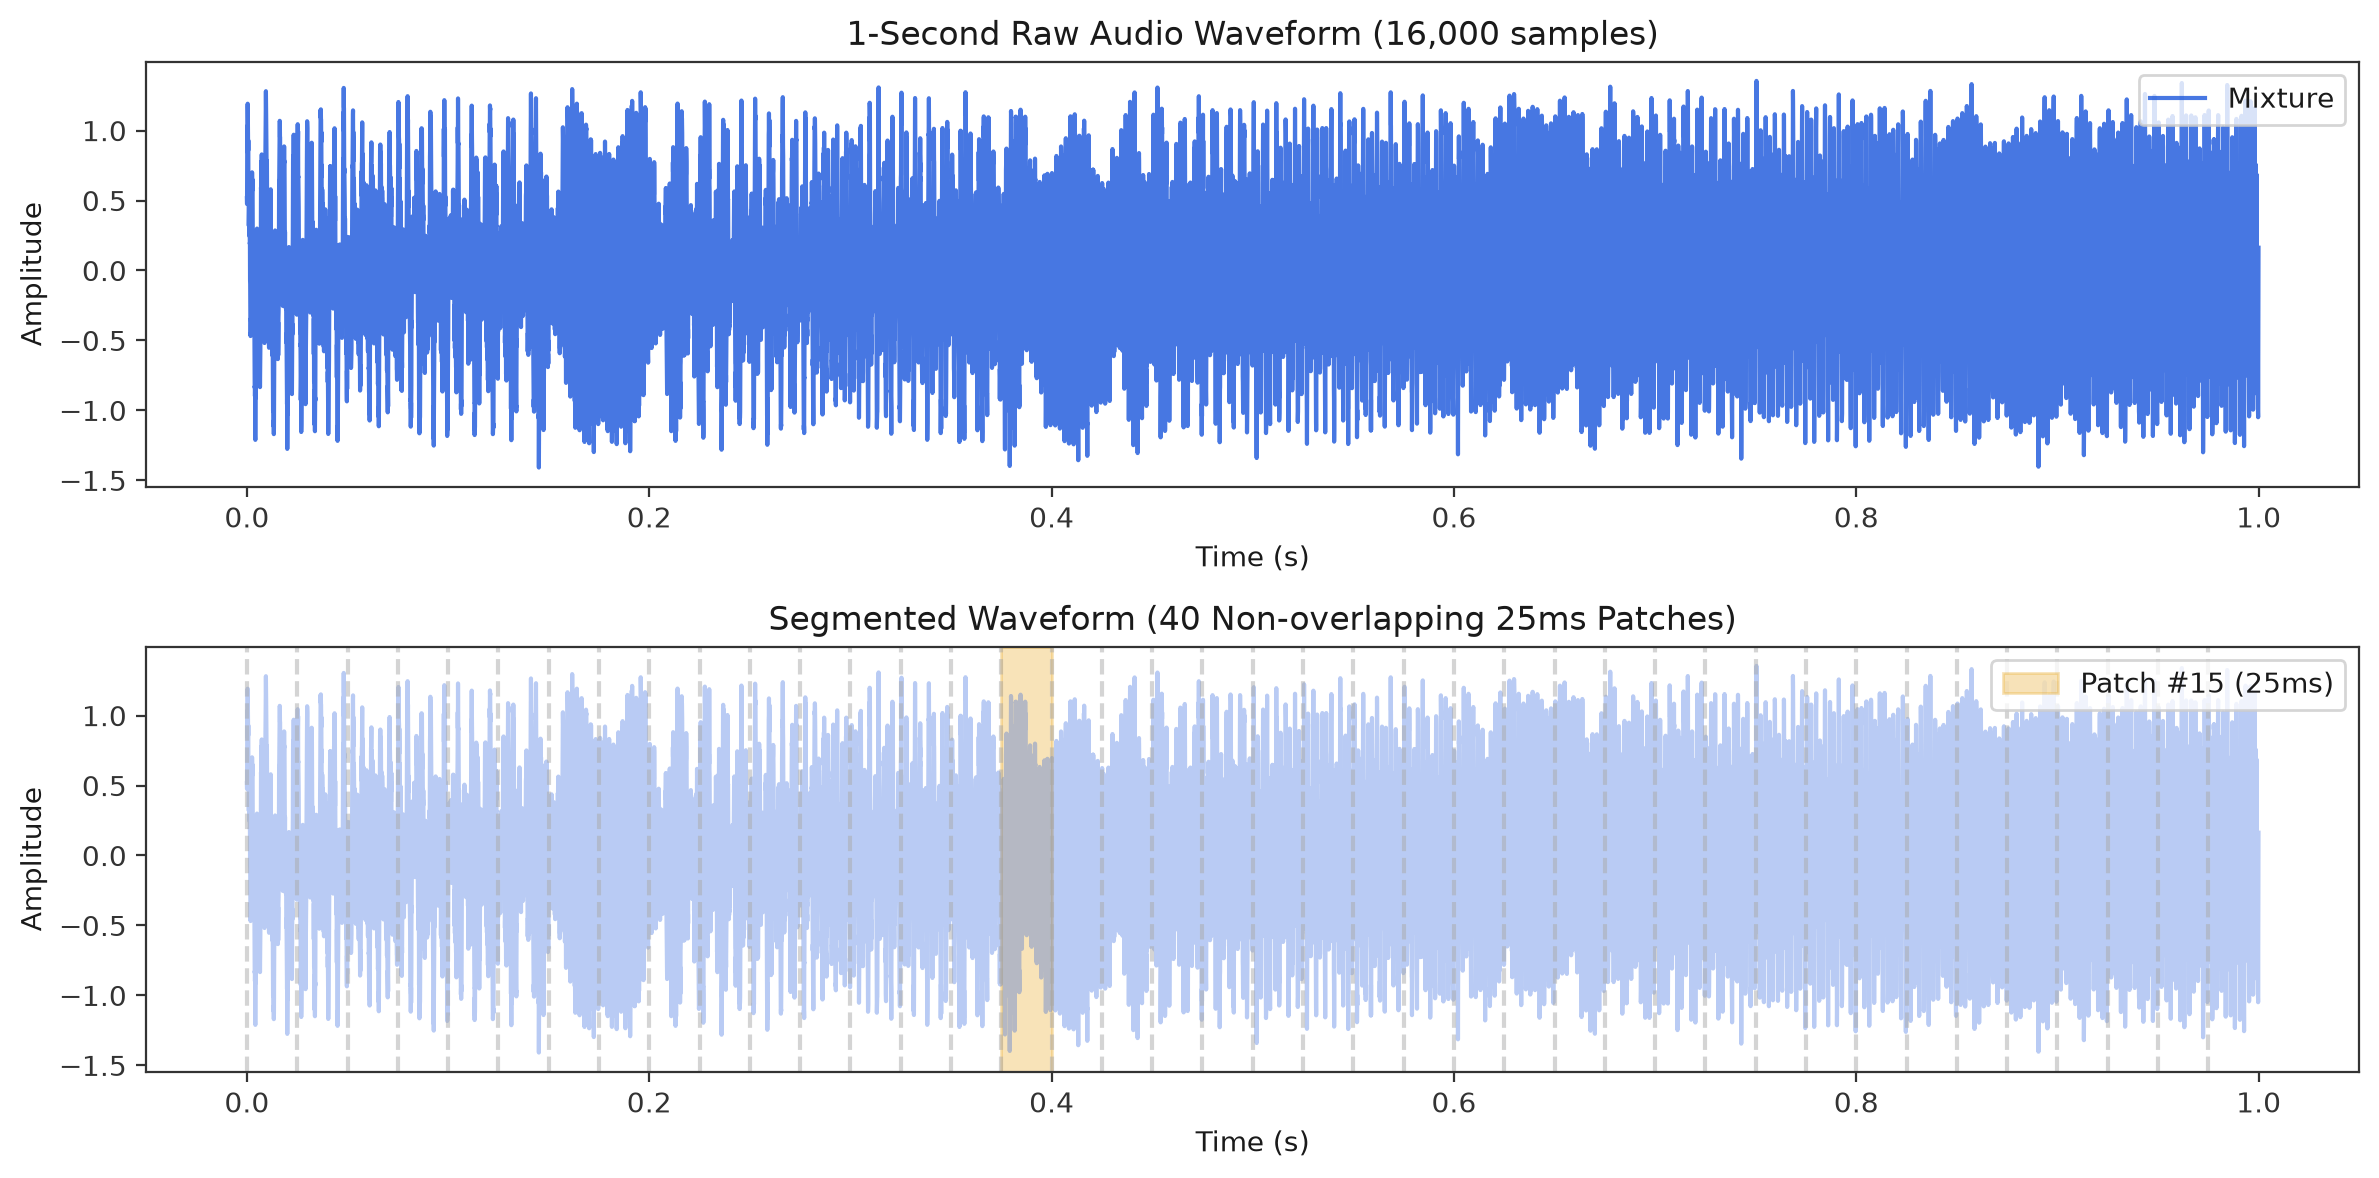
\includegraphics[width=0.95\columnwidth]{waveform_patching.png}
\caption{Raw 1-second audio waveform (16,000 samples) segmented into 40 non-overlapping 25ms patches. Patch \#15 is highlighted in yellow.}
\label{fig:waveform_patching}
\end{figure}

\subsection{Emergent Biological Filterbanks}
During training, the 2048 weights in the FC layer self-organize into a problem-specific, non-constant bandwidth filterbank. Simulation of these weights reveals that the network autonomously rediscovers fundamental acoustic processing strategies analogous to the basilar membrane:
\begin{enumerate}
    \item \textbf{Sinusoidal Basis Functions:} Sharp, frequency-tuned detectors for harmonic analysis.
    \item \textbf{Hanning/Hamming Windows:} Tapered envelopes that suppress spectral leakage at patch boundaries.
    \item \textbf{Onset Detectors:} Asymmetric transient spikes for detecting consonants and percussive events.
    \item \textbf{Energy Envelopes:} Low-frequency integrators capturing overall volume dynamics.
\end{enumerate}
This demonstrates that neural networks, when given raw temporal data, will naturally converge on physical principles of sound analysis.

\begin{figure}[htbp]
\centering
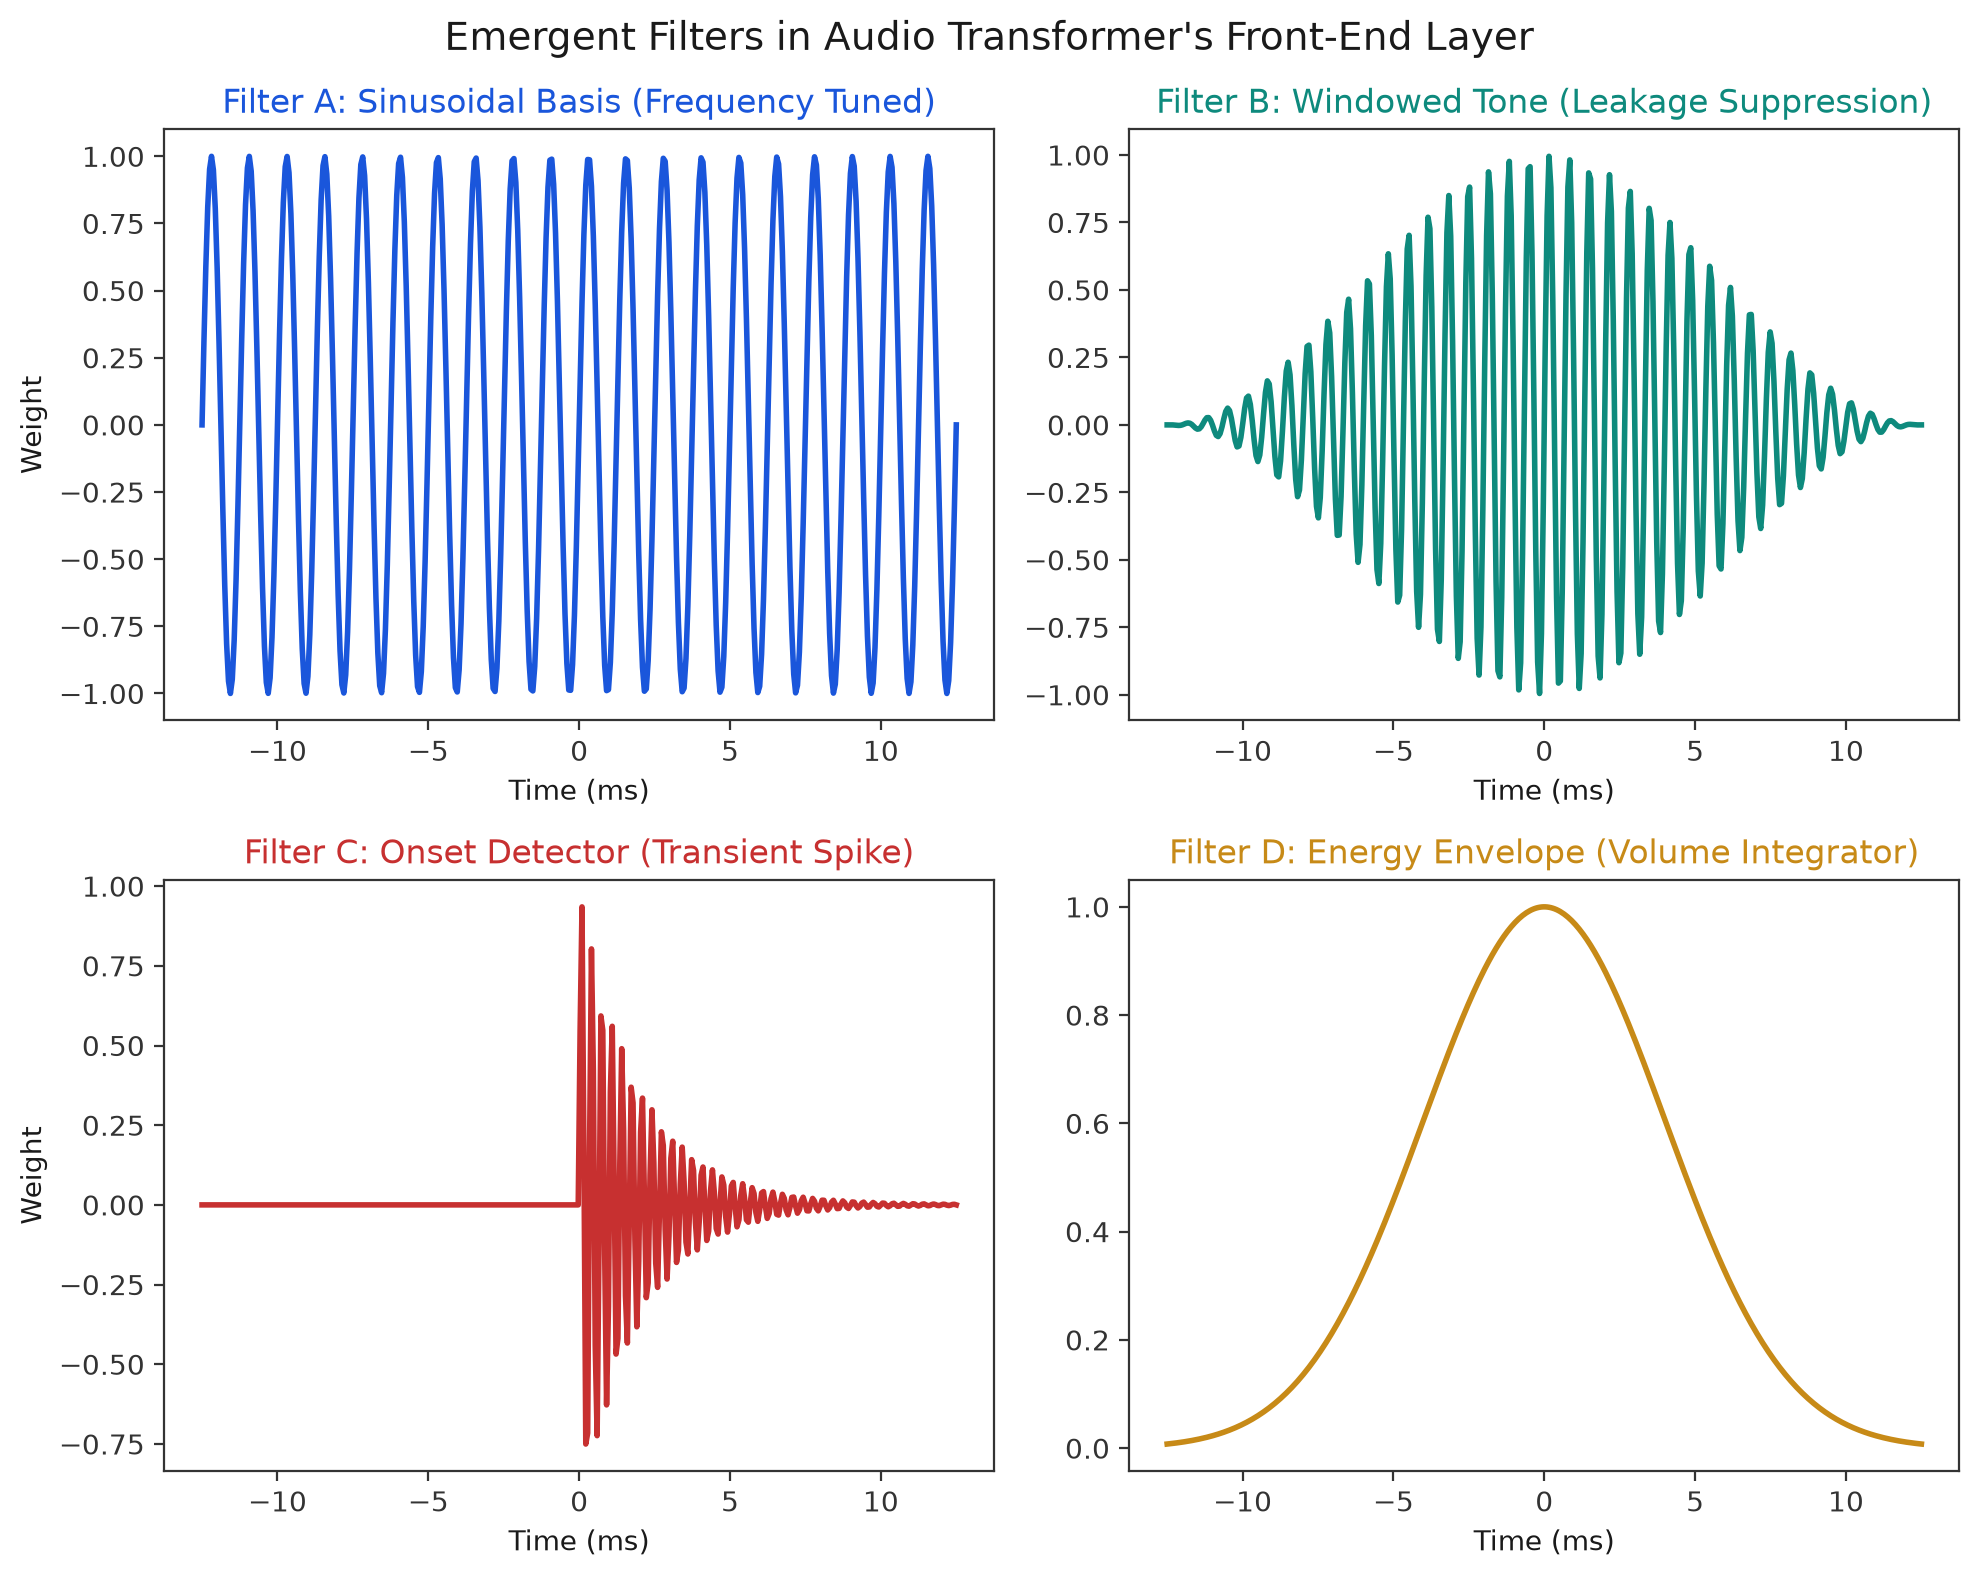
\includegraphics[width=0.95\columnwidth]{learned_filterbanks.png}
\caption{Emergent filters in the Audio Transformer's front-end layer. (A) Sinusoidal basis for harmonic analysis, (B) Windowed tone for leakage suppression, (C) Onset detector for transient events, (D) Energy envelope for volume integration.}
\label{fig:learned_filterbanks}
\end{figure}

\begin{figure*}[tbp]
\centering
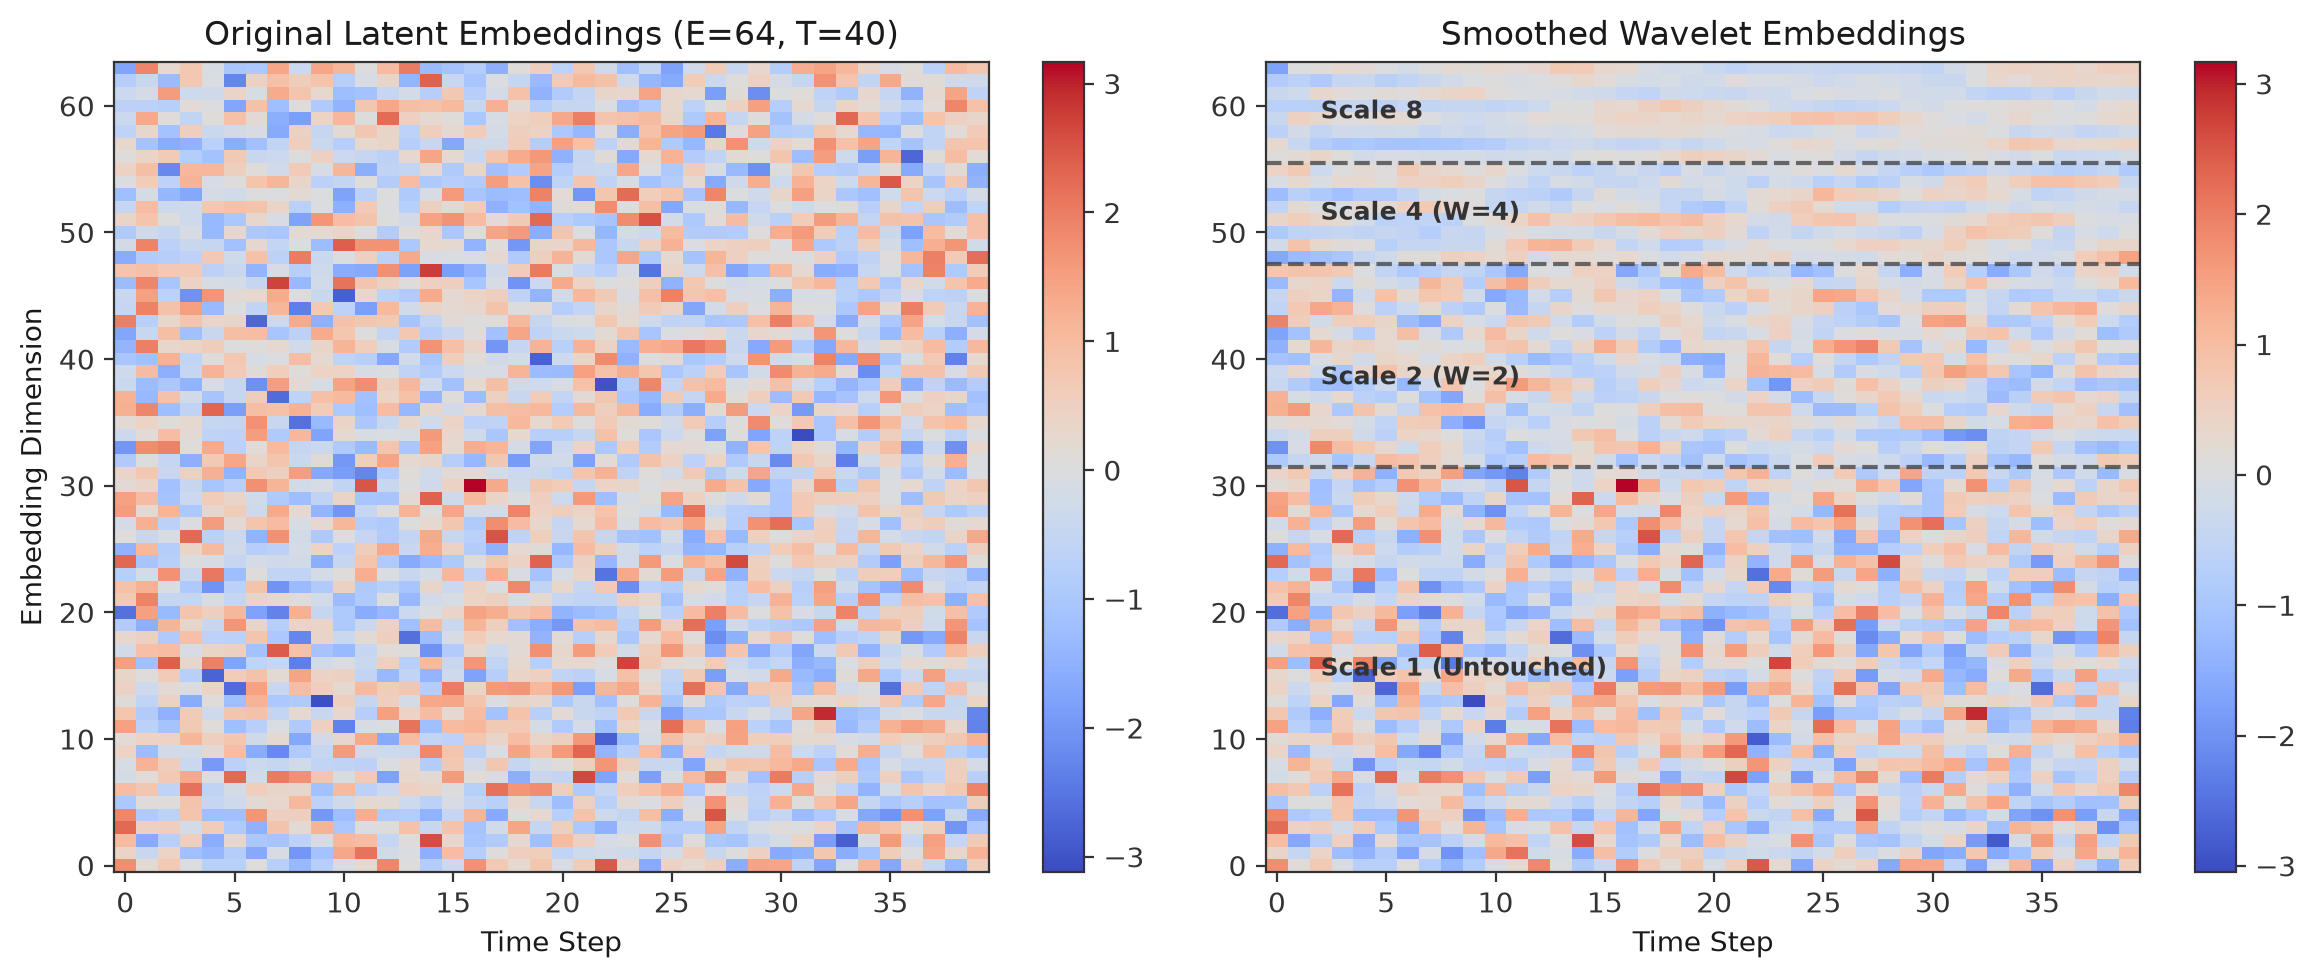
\includegraphics[width=0.9\textwidth]{wavelet_embeddings.png}
\caption{Multi-scale wavelet embedding decomposition. (Left) Original latent embeddings ($E=64$, $T=40$). (Right) After wavelet smoothing, with dimensions partitioned into four temporal scales (Scale 1: untouched, Scale 2: $W=2$, Scale 4: $W=4$, Scale 8: $W=8$).}
\label{fig:wavelet_embeddings}
\end{figure*}

\section{Auditory Object Permanence via Self-Distillation}

\subsection{The Psychology of Illusory Continuation}
When a continuous tone is interrupted by a brief gap of silence, human listeners accurately perceive the gap. However, if that gap is filled with a loud burst of broad-spectrum noise, listeners report hearing the tone continue uninterrupted \textit{behind} the noise. This phenomenon, known as illusory continuation or auditory object permanence, proves that hearing is a generative, predictive process rather than a passive feed-forward mechanism.

\subsection{DINO as a Model for Predictive Hearing}
The DINO (Self-Distillation with No Labels) framework~\cite{b2}, originally designed for Vision Transformers, provides a rigorous mathematical model for this cognitive phenomenon. DINO aligns a Student network's prediction of a global context (from a local or masked view) with a Teacher network's output (representing the unmasked global view).

The loss function minimizes the cross-entropy between the Student and Teacher probabilities:
\begin{equation}
    \mathcal{L} = - \sum_{k} P_{\text{teacher}}(k) \log P_{\text{student}}(k)
\end{equation}

To prevent representational collapse, the framework utilizes \textit{centering} (subtracting a running mean) and \textit{sharpening} (temperature scaling $\tau_s < \tau_t$). 

By forcing the Student to predict the Teacher's representation of an unmasked audio clip from a masked (or noise-filled) patch, the network learns to infer missing acoustic data. The Student's output is therefore mathematically equivalent to the brain's predictive percept of the continuous tone beneath the noise burst.

\begin{figure}[htbp]
\centering
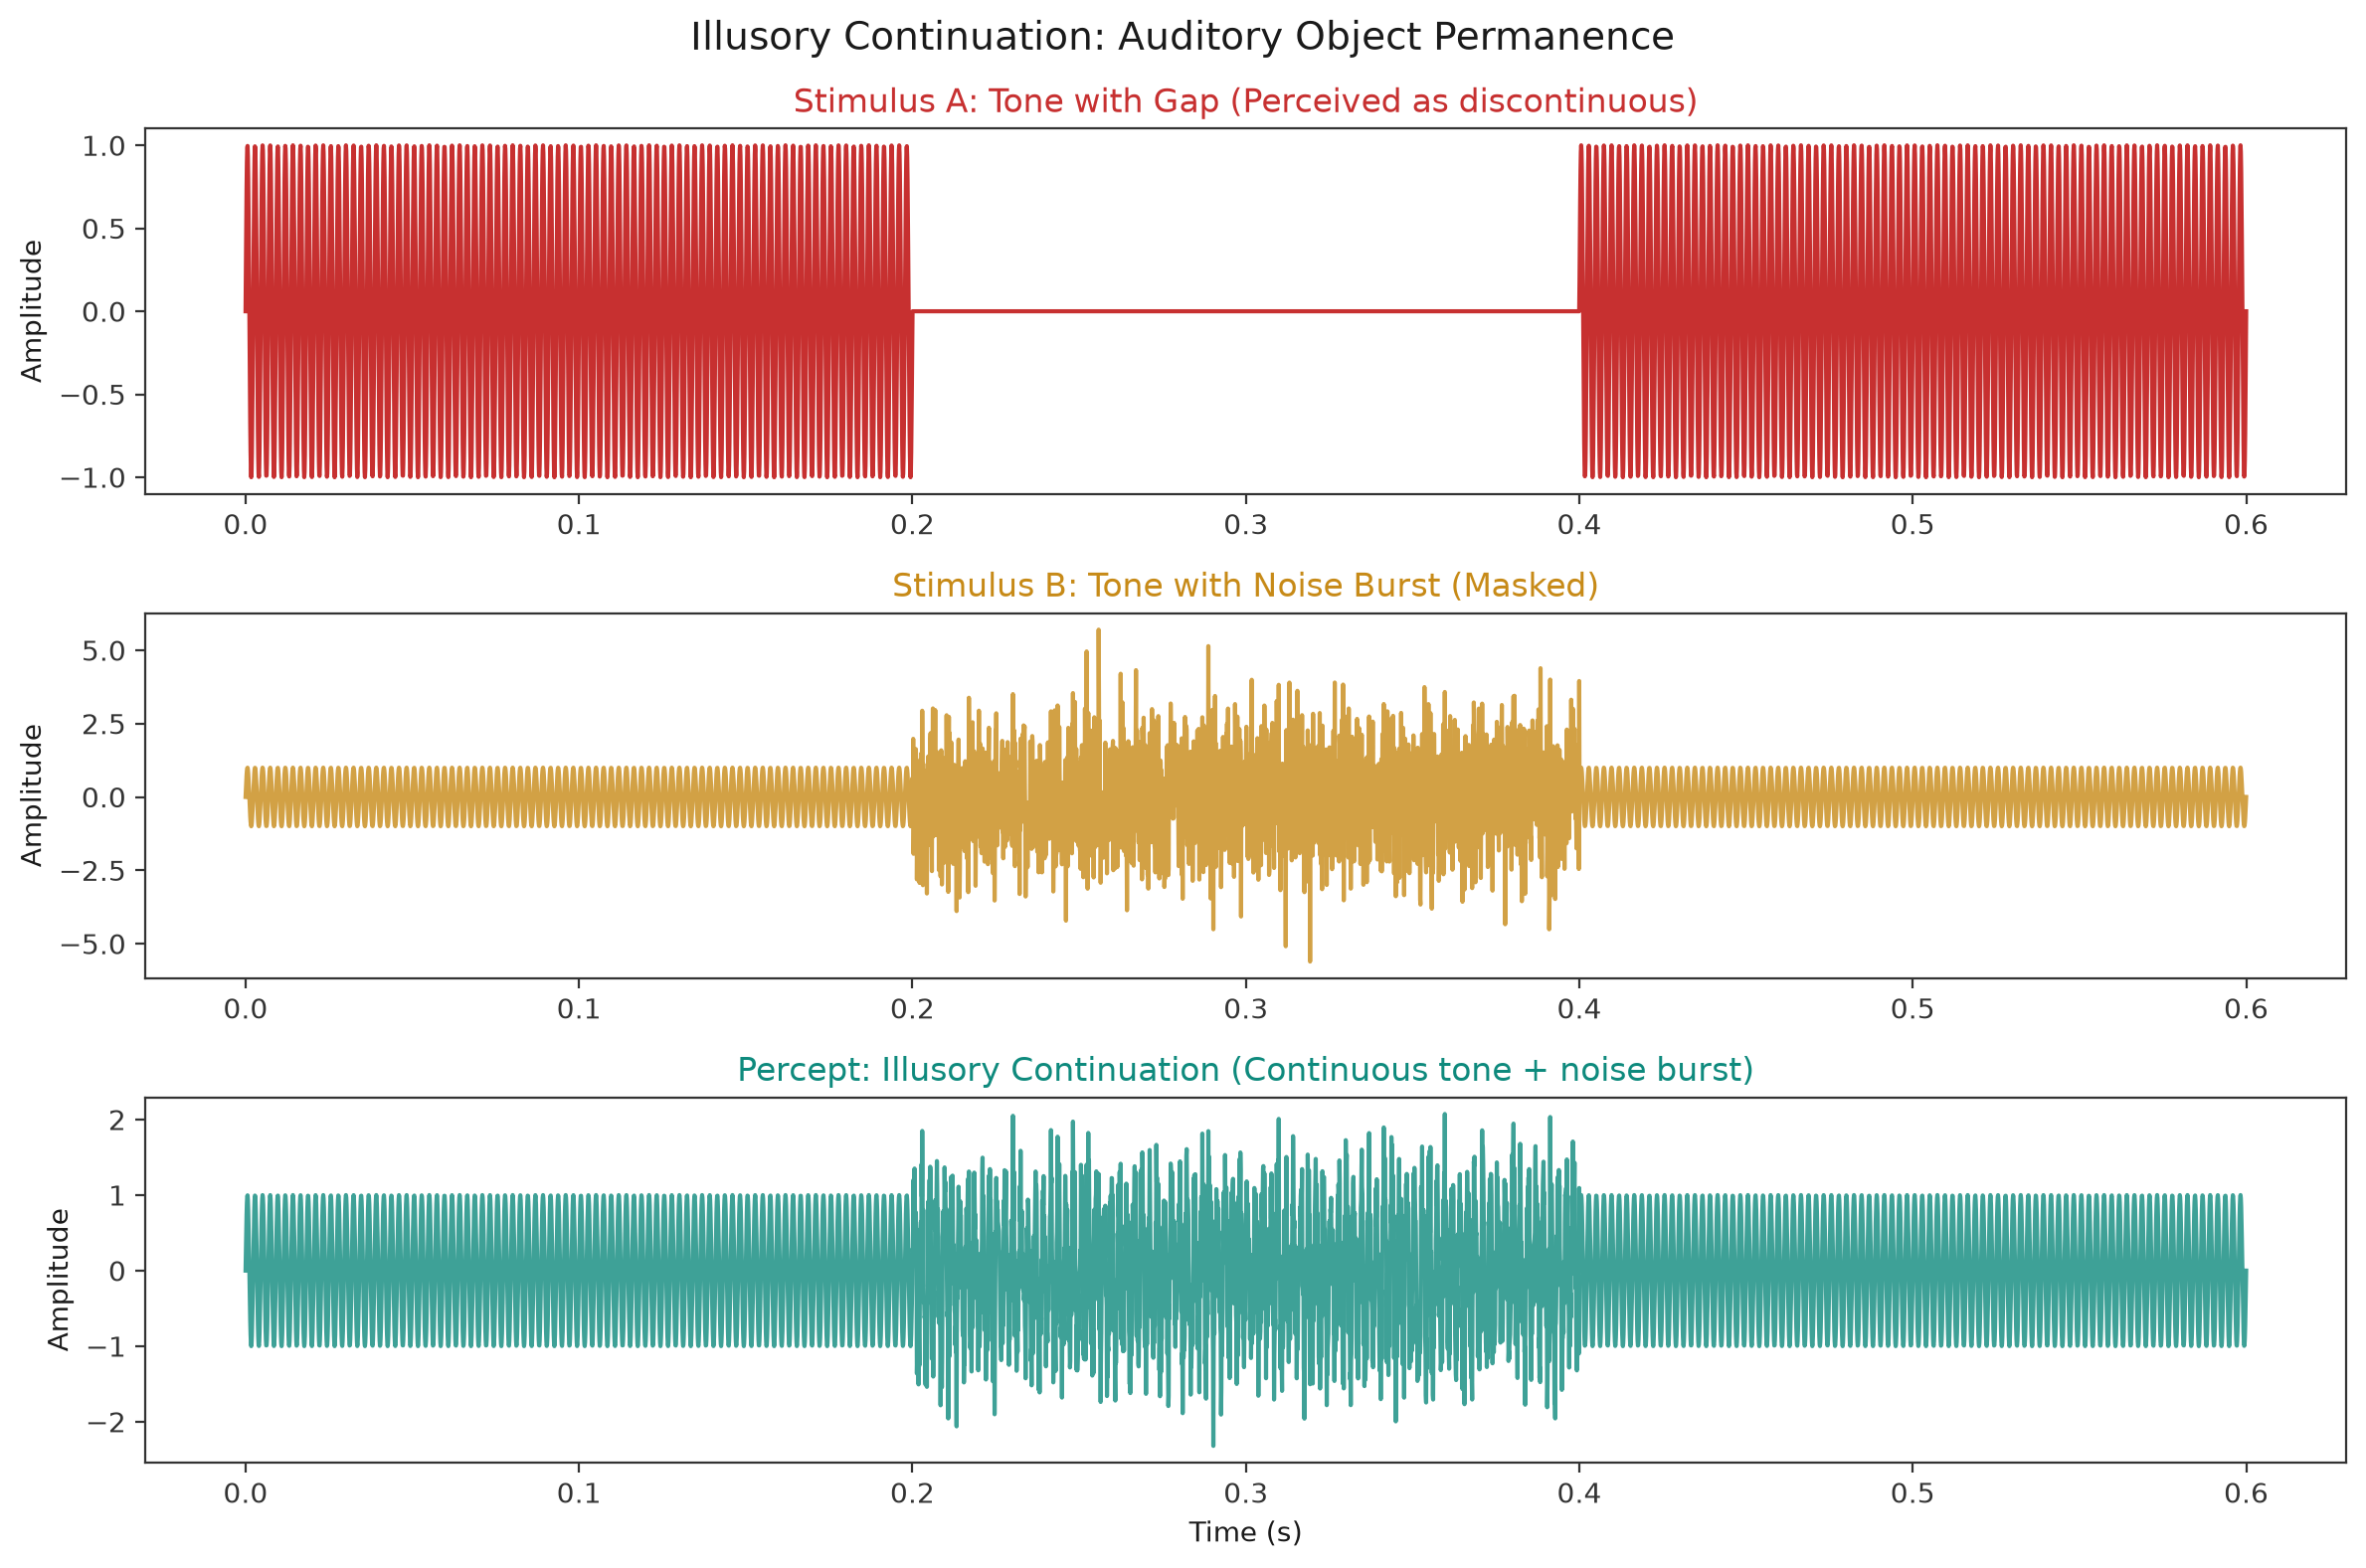
\includegraphics[width=0.95\columnwidth]{illusory_continuation.png}
\caption{Illusory continuation simulation. (Top) A tone with a silent gap is perceived as discontinuous. (Middle) The same gap filled with noise masks the discontinuity. (Bottom) The brain's percept: the tone is heard as continuous \textit{behind} the noise burst---auditory object permanence.}
\label{fig:illusory_continuation}
\end{figure}

\section{Cochlear Self-Attention and Discretization}

\subsection{Top-Down Efferent Tuning}
Vision Transformers utilize self-attention maps to segment salient visual objects. In the auditory domain, we apply self-attention over the time-frequency cochleagram. Simulations reveal that individual attention heads specialize dynamically: one head tracks continuous pitch glides (vowels), while another binds exclusively to transient bursts (consonants). 

Biologically, this mirrors the brain's efferent feedback pathways, where the cortex sends signals back down to the cochlea to physically tune the sensitivity of outer hair cells, focusing attention on a specific voice in a crowded room.

\begin{figure}[htbp]
\centering
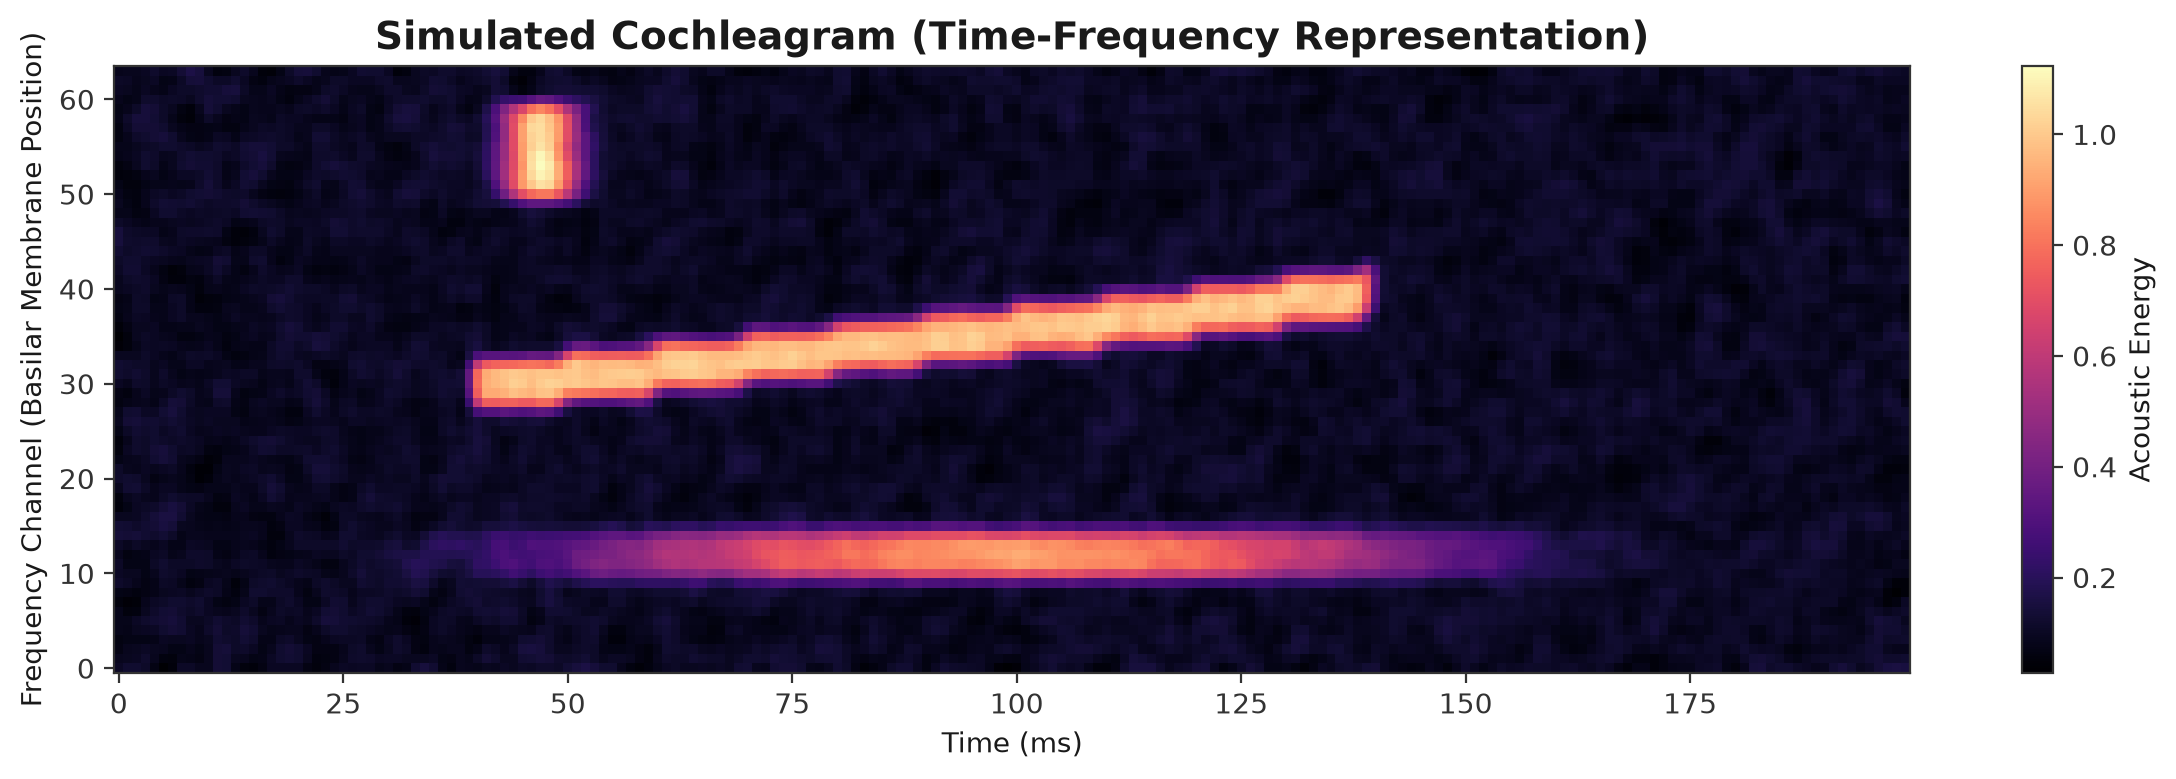
\includegraphics[width=0.95\columnwidth]{cochleagram.png}
\caption{Simulated cochleagram showing time-frequency acoustic energy. Three distinct auditory objects are visible: a sustained low-frequency formant, a gliding mid-frequency pitch contour, and a high-frequency transient burst.}
\label{fig:cochleagram}
\end{figure}

\begin{figure*}[tbp]
\centering
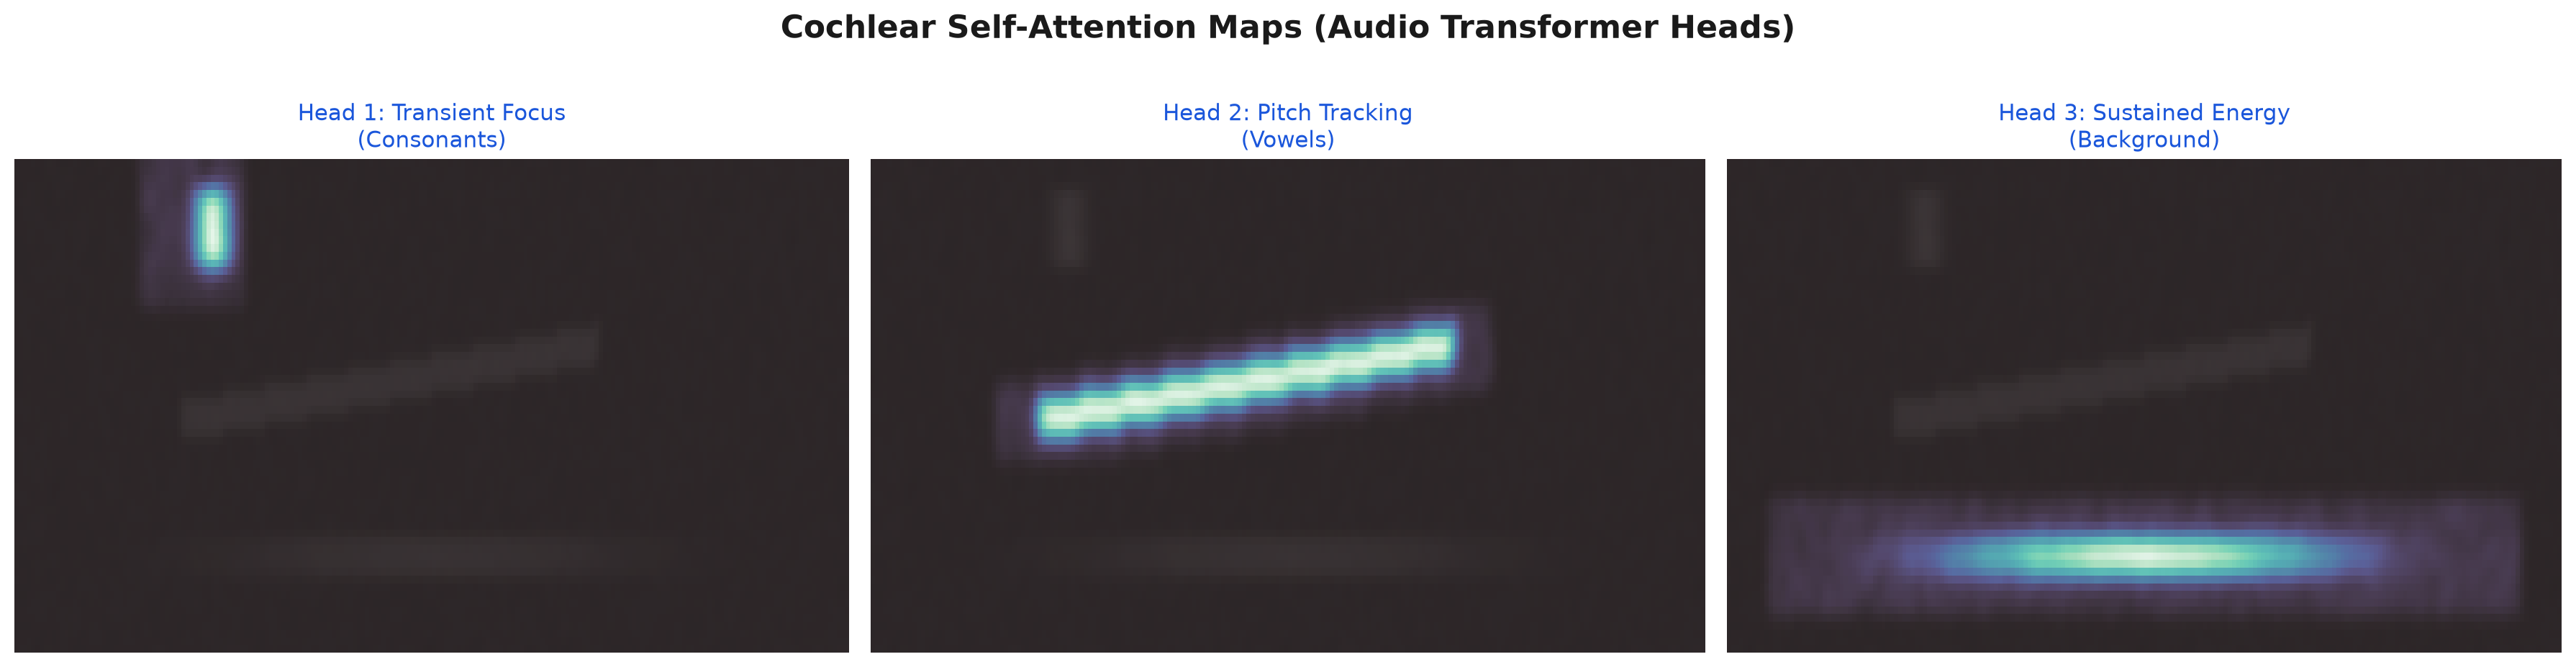
\includegraphics[width=0.95\textwidth]{cochlear_attention.png}
\caption{Cochlear Self-Attention Maps. Three simulated attention heads dynamically bind to distinct acoustic objects in the cochleagram: Head 1 focuses on transient consonant bursts, Head 2 tracks the gliding pitch of vowels, and Head 3 attends to sustained low-frequency energy.}
\label{fig:cochlear_attention}
\end{figure*}

\subsection{The Mimi Codec as the Auditory Nerve}
Modern neural voice architectures, such as the TinyAya speech-to-speech model~\cite{b4}, rely on quantization codecs (e.g., Mimi) to compress continuous audio embeddings into discrete tokens (Codebooks CB0-CB7) at specific frame rates (e.g., 12.5 Hz).

This mechanism is perfectly isomorphic to the human auditory nerve. The auditory nerve translates continuous acoustic pressure gradients from the cochlea into discrete, all-or-nothing action potentials (spike trains). By mapping the continuous outputs of our learned audio frontend through a quantization layer, we simulate the discretization bottleneck that defines human sensory encoding.

\begin{figure}[htbp]
\centering
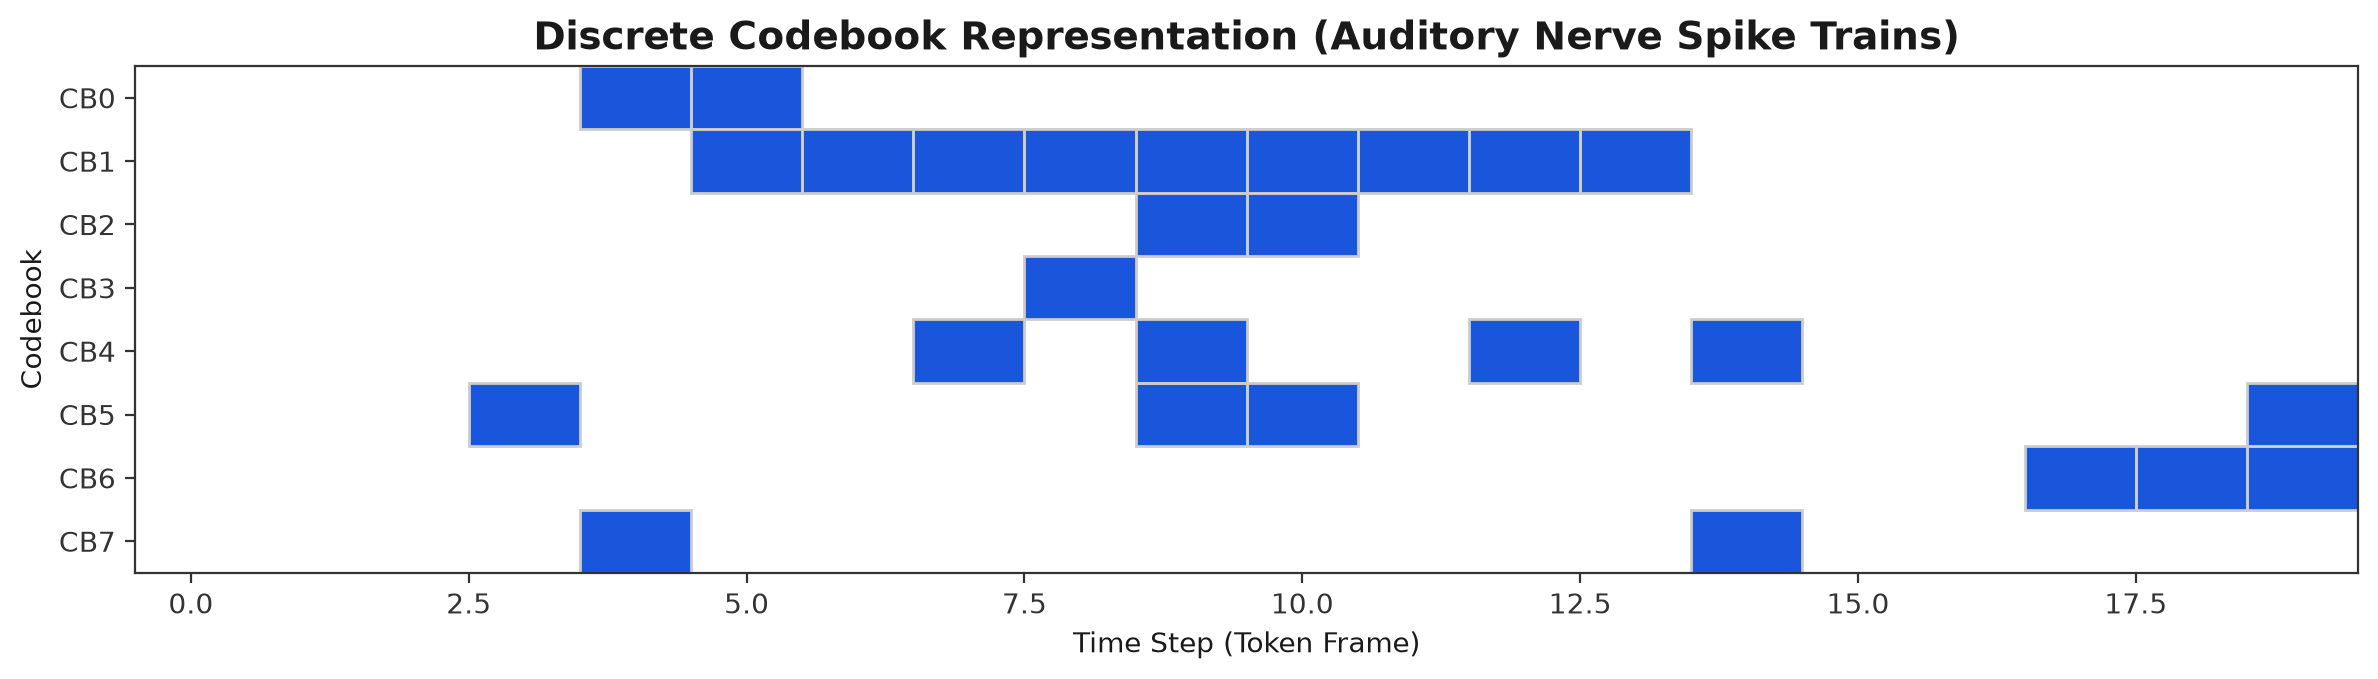
\includegraphics[width=0.95\columnwidth]{codebook_spikes.png}
\caption{Discrete codebook representation simulating auditory nerve spike trains. CB0--CB2 track the three attention heads (transients, formants, sustained energy), while CB3--CB7 represent stochastic neural noise.}
\label{fig:codebook_spikes}
\end{figure}

\section{Language Cortex Parallel Streams}

A critical challenge in human interaction is the ability to listen and plan speech simultaneously. Wernicke's area (reception) and Broca's area (production) must operate concurrently, connected by the arcuate fasciculus.

The Cohere 3B Backbone within the TinyAya architecture models this through a \textit{Parallel Two-Stream Format}. The network ingests the discrete tokens from the user's audio stream (listening) while simultaneously maintaining an internal semantic state that drives a parallel model audio stream (speaking/planning).

Simulations of this architecture demonstrate robust turn-taking behavior. As the user stream peaks, the model stream remains silent while an internal semantic planning vector accumulates energy, eventually triggering the output stream once the user pauses. This provides a compelling computational model for conversational cognitive dynamics.

\begin{figure}[htbp]
\centering
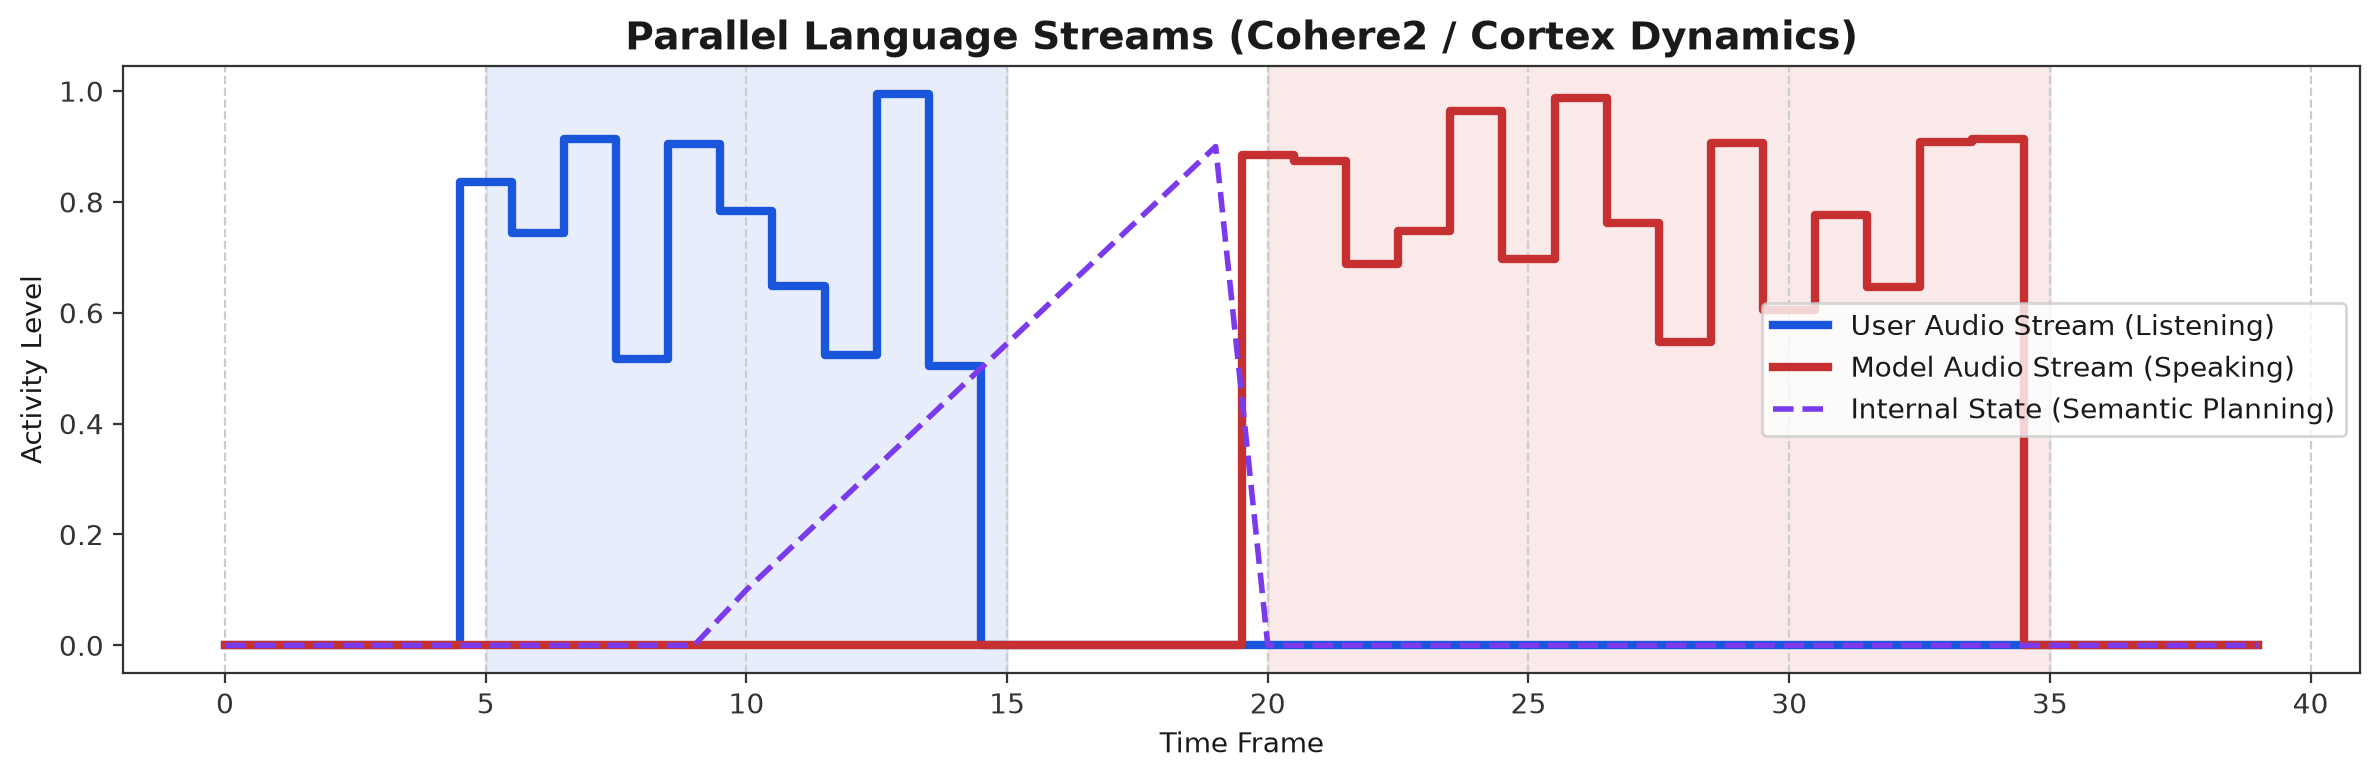
\includegraphics[width=0.95\columnwidth]{parallel_streams.png}
\caption{Parallel language streams simulation modeling the Wernicke-Broca cortex loop. The User Audio Stream (blue, listening) and Model Audio Stream (red, speaking) alternate, mediated by an Internal Semantic Planning state (purple, dashed) that accumulates during listening.}
\label{fig:parallel_streams}
\end{figure}

\section{Spectral Transform Units: Fixed Filters from Hankel Eigendecomposition}

While the Audio Transformer learns its filterbank from data, a complementary approach exists: the \textit{Spectral State Space Model} (Spectral SSM)~\cite{b5}, which uses \textbf{fixed} convolutional filters derived from the eigendecomposition of a Hankel matrix. Its optimized implementation, Flash STU~\cite{b6}, combines these fixed spectral filters with Flash FFT convolutions for efficient long-range sequence modeling.

\subsection{The Spectral Hankel Matrix}
The Spectral SSM constructs a Hankel matrix $Z \in \mathbb{R}^{n \times n}$:
\begin{equation}
    Z_{i,j} = \frac{2}{(i+j)^3 - (i+j)}
\end{equation}

The top-$k$ eigenvectors $\phi_1, \ldots, \phi_k$ of $Z$ serve as fixed convolutional filters. These filters are \textit{never trained}---they are derived purely from the mathematical structure of autocovariance in sequences.

\begin{figure}[htbp]
\centering
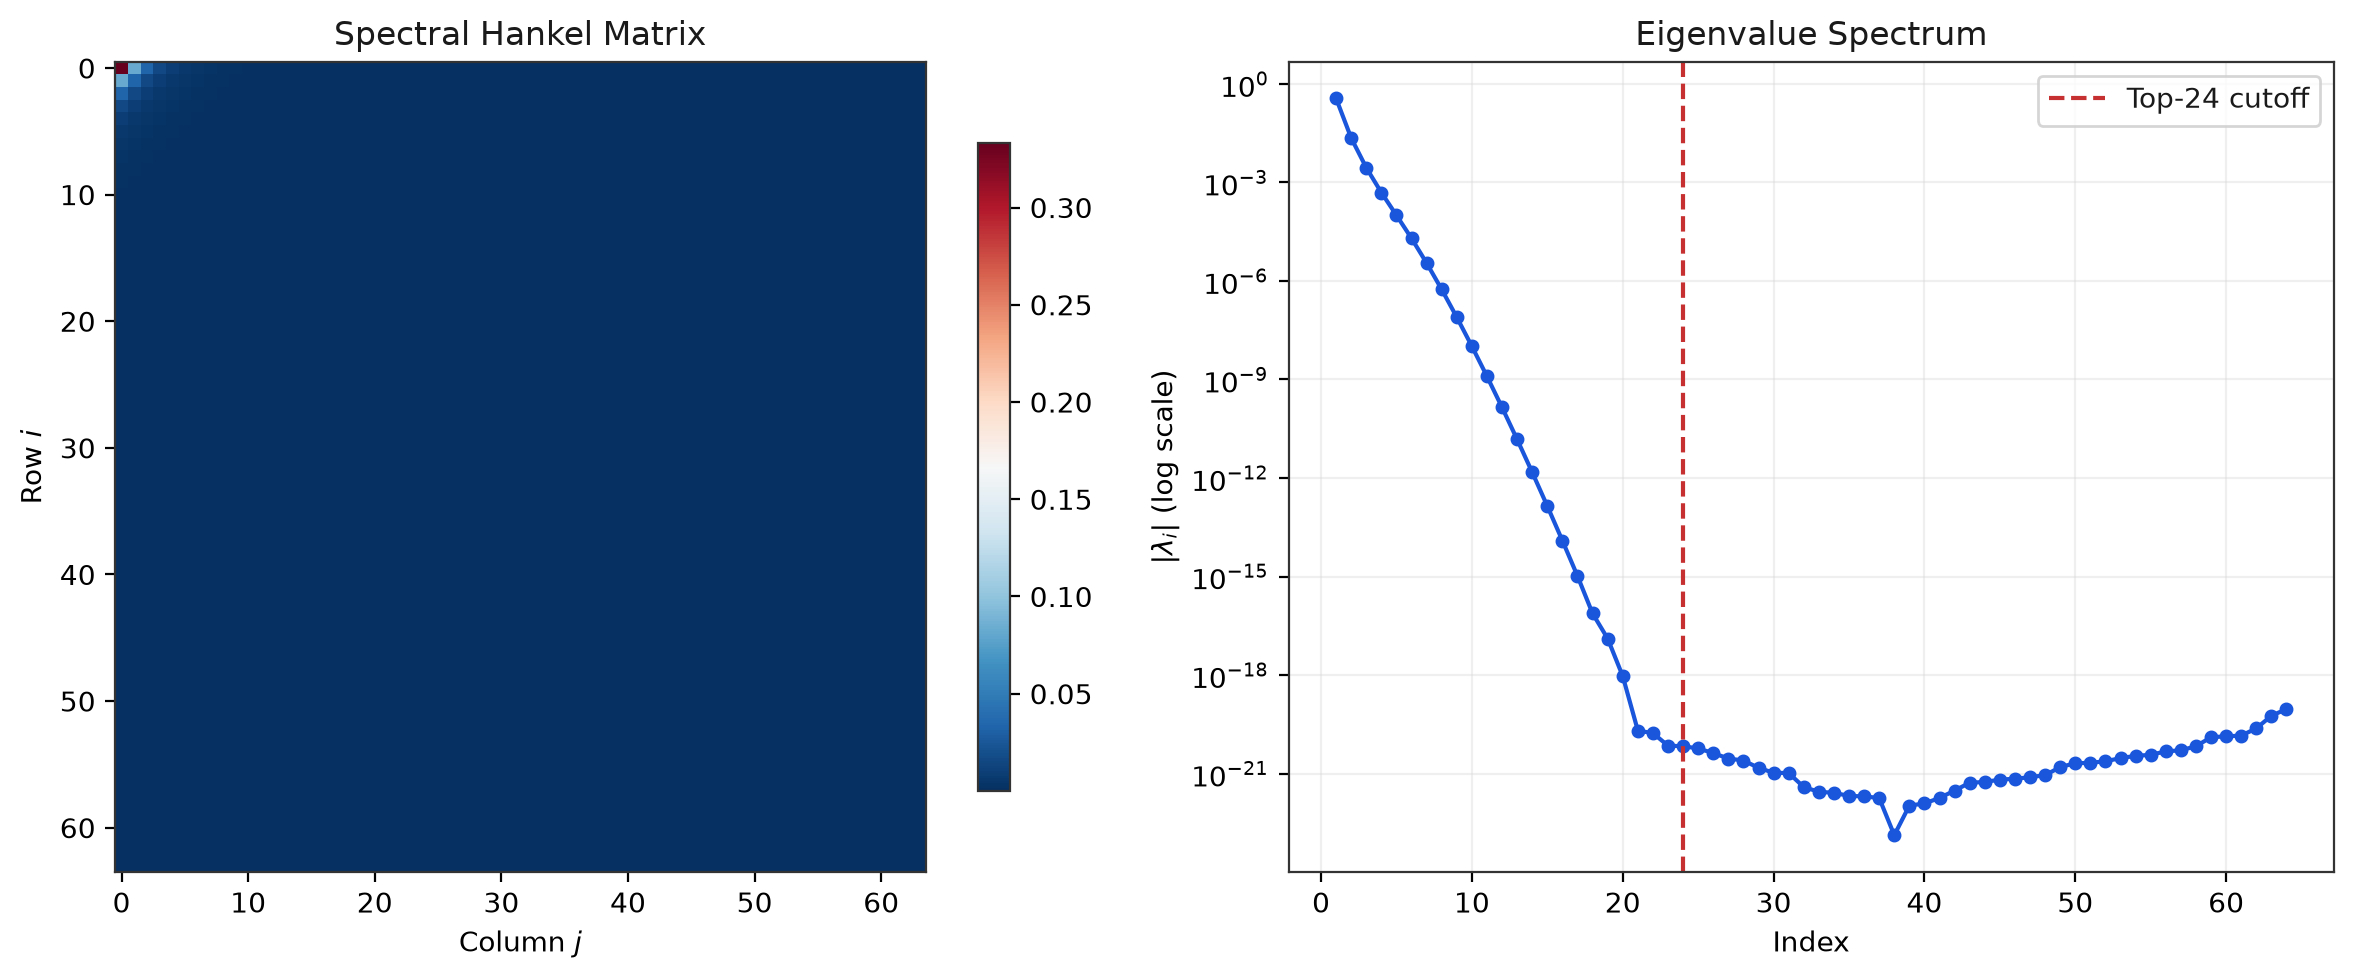
\includegraphics[width=0.95\columnwidth]{hankel_eigenspectrum.png}
\caption{(Left) The spectral Hankel matrix $Z_{i,j}$. (Right) Eigenvalue spectrum showing rapid decay; the top-24 eigenvalues (left of the red line) capture the dominant temporal structure.}
\label{fig:hankel}
\end{figure}

\subsection{Cochlear Resonance as Fixed Spectral Filtering}
The basilar membrane in the cochlea is a \textit{physically fixed} resonant structure whose frequency selectivity is determined by mechanical properties (stiffness, mass, damping), not by neural learning. Its impulse response at characteristic frequency $f_c$ is:
\begin{equation}
    h(t) = e^{-\gamma t} \sin(2\pi f_c t)
\end{equation}

Remarkably, the Hankel eigenvectors exhibit the same structural pattern: the top eigenvectors are smooth and slowly varying (like apical cochlear resonances at low frequencies), while lower eigenvectors are fast and oscillatory (like basal resonances at high frequencies). This correspondence is not coincidental---both arise from the spectral decomposition of a physical or mathematical operator.

\begin{figure*}[tbp]
\centering
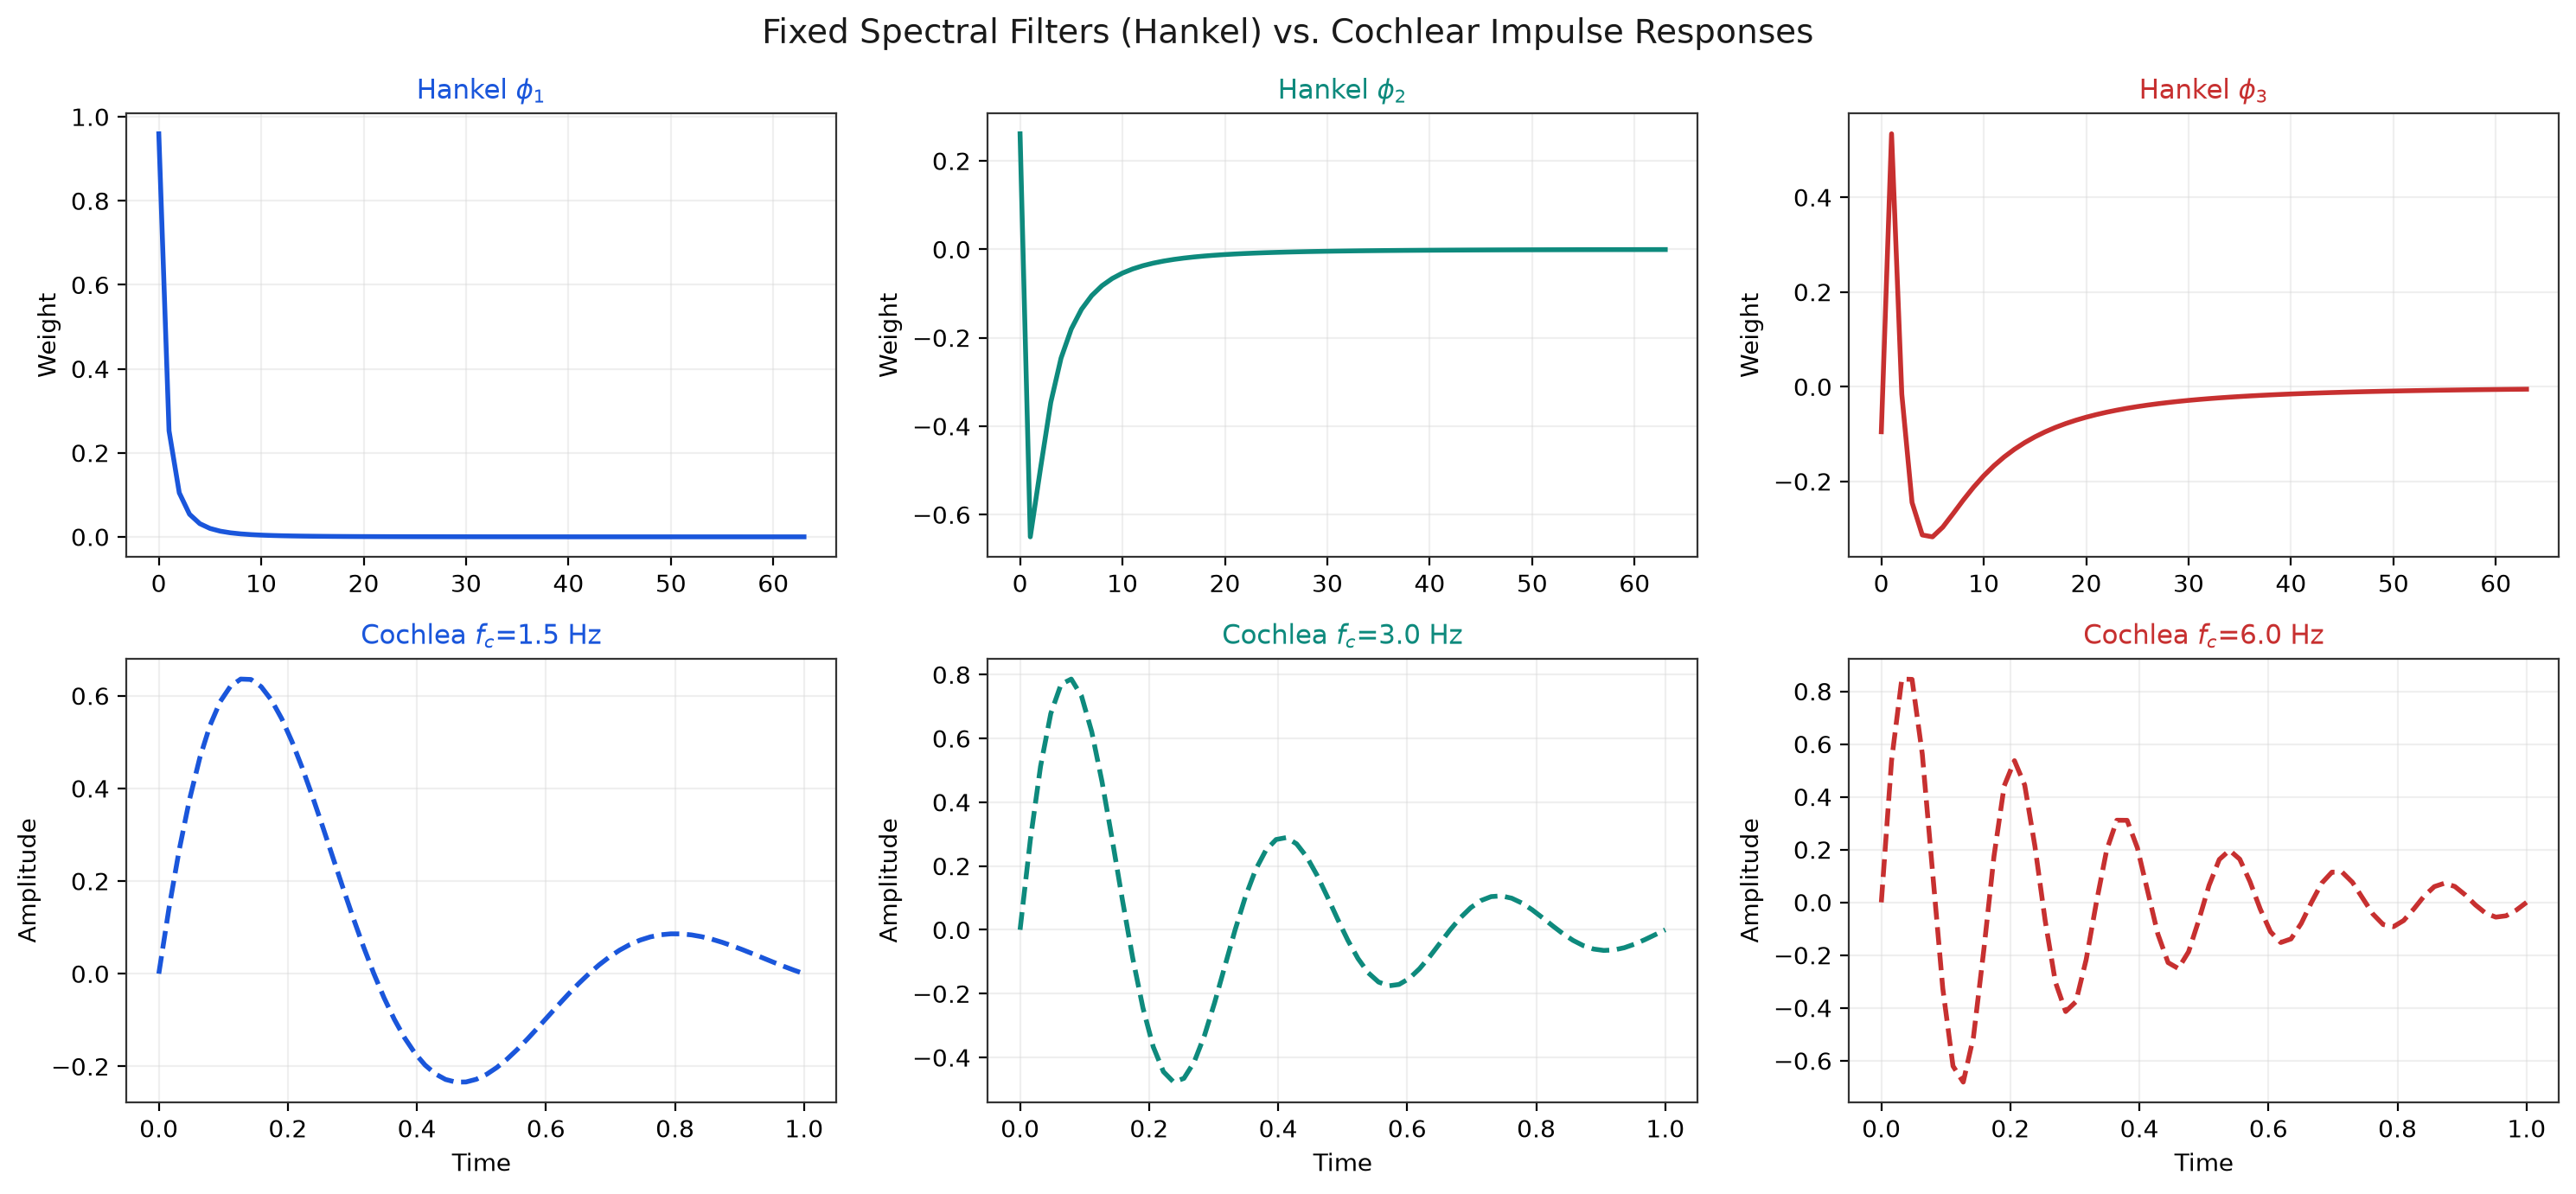
\includegraphics[width=0.95\textwidth]{hankel_vs_cochlea.png}
\caption{Structural correspondence between fixed Hankel eigenvectors (top row) and simulated cochlear impulse responses (bottom row). Both exhibit the same progression from slow, smooth temporal modes to fast, oscillatory modes---without any training.}
\label{fig:hankel_cochlea}
\end{figure*}

\subsection{Three Paradigms of Auditory Frontends}
The Spectral SSM completes a taxonomy of auditory processing paradigms. (1) \textit{Fixed Spectral}: Hankel eigenvectors that are structurally determined, analogous to the basilar membrane. (2) \textit{Learned}: Audio Transformer filterbanks trained end-to-end, analogous to efferent cochlear tuning. (3) \textit{Self-Supervised}: DINO-style distillation, analogous to predictive coding and illusory continuation. In practice, the STU combines fixed spectral filters with a small learned autoregressive component, mirroring biology's combination of fixed cochlear mechanics and adaptive cortical processing.

\section{Sociotechnical Implications}

The convergence of high-fidelity local text-to-speech (e.g., Browser-Speech utilizing Pocket TTS) with predictive, parallel-stream translation models raises significant sociotechnical questions. 

Unlike previous generations of cloud-based APIs, these models run entirely locally, democratizing access to neural voice synthesis but also enabling undetectable, zero-latency spoofing. Furthermore, by designing architectures that mimic biological listening (e.g., implementing auditory object permanence and cocktail party segregation), we create machines capable of superhuman acoustic surveillance. 

As we refine these cyber-physical frameworks, we must prioritize cryptographic provenance and hardware-level acoustic watermarking to preserve trust in digital audio.

\section{Conclusion}

By deconstructing the components of Audio Transformers, Neural Voice models, and Spectral State Space Models and mapping them onto biological structures, we provide a unified framework for understanding machine hearing. Fixed spectral filters mirror the cochlea's physically determined resonance, learnable filterbanks mirror efferent tuning, self-supervised distillation explains illusory continuation, quantization codecs model the auditory nerve, and parallel streams replicate the language cortex. This synthesis bridges deep learning, dynamical systems theory, and cognitive psychology, offering a blueprint for more resilient, human-like auditory AI.

\begin{thebibliography}{00}
\bibitem{b1} P. Verma and J. Berger, ``Audio Transformers: Transformer Architectures for Large Scale Audio Understanding. Adieu Convolutions,'' \emph{arXiv preprint arXiv:2105.00335}, 2021.

\bibitem{b2} M. Caron, H. Touvron, I. Misra, H. Jégou, J. Mairal, P. Bojanowski, and A. Joulin, ``Emerging Properties in Self-Supervised Vision Transformers,'' \emph{arXiv preprint arXiv:2104.14294}, 2021.

\bibitem{b3} Kyutai, ``Pocket TTS: High-quality, fully local text-to-speech,'' \emph{Browser-Speech Documentation}, 2026.

\bibitem{b4} Cohere Labs, ``TinyAya: Moshi-style speech-to-speech translation model,'' \emph{GitHub Repository}, 2026.

\bibitem{b5} N. Agarwal, D. Suo, X. Chen, and E. Hazan, ``Spectral State Space Models,'' \emph{arXiv preprint arXiv:2312.06837}, 2024.

\bibitem{b6} Y. I. Liu, W. Nguyen, Y. Devre, E. Dogariu, A. Majumdar, and E. Hazan, ``Flash STU: Fast Spectral Transform Units,'' \emph{arXiv preprint arXiv:2409.10489}, 2024.
\end{thebibliography}

\end{document}

